% \iffalse
\let\negmedspace\undefined
\let\negthickspace\undefined
\documentclass[journal,12pt,twocolumn]{IEEEtran}
\usepackage{cite}
\usepackage{amsmath,amssymb,amsfonts,amsthm}
\usepackage{algorithmic}
\usepackage{graphicx}
\usepackage{textcomp}
\usepackage{xcolor}
\usepackage{txfonts}
\usepackage{listings}
\usepackage{enumitem}
\usepackage{mathtools}
\usepackage{gensymb}
\usepackage{comment}
\usepackage[breaklinks=true]{hyperref}
\usepackage{tkz-euclide} 
\usepackage{listings}
\usepackage{gvv}                                        
\def\inputGnumericTable{}                                 
\usepackage[latin1]{inputenc}                                
\usepackage{color}                                            
\usepackage{array}                                            
\usepackage{longtable}                                       
\usepackage{calc}                                             
\usepackage{multirow}                                         
\usepackage{hhline}                                           
\usepackage{ifthen}                                           
\usepackage{lscape}
\usepackage{placeins}
\usepackage{xparse}


\newtheorem{theorem}{Theorem}[section]
\newtheorem{problem}{Problem}
\newtheorem{proposition}{Proposition}[section]
\newtheorem{lemma}{Lemma}[section]
\newtheorem{corollary}[theorem]{Corollary}
\newtheorem{example}{Example}[section]
\newtheorem{definition}[problem]{Definition}
\newcommand{\BEQA}{\begin{eqnarray}}
\newcommand{\EEQA}{\end{eqnarray}}
\newcommand{\define}{\stackrel{\triangle}{=}}
\theoremstyle{remark}
\newtheorem{rem}{Remark}

\begin{document}

\bibliographystyle{IEEEtran}
\vspace{3cm}

\Large\title{NCERT Question 10.5.2.5}
\large\author{EE23BTECH11032 - Kaustubh Parag Khachane $^{*}$% <-this % stops a space
}
\maketitle
\newpage
\bigskip

\renewcommand{\thefigure}{\theenumi}
\renewcommand{\thetable}{\theenumi}
\large\textbf{Question 10.5.2.5} : \normalsize Find the number of terms in each of the following APs : 

\brak{i} 7, 13, 19, ... 205

\brak{ii} 18, 15$\frac{1}{2}$, 13, ... -47

\vspace{4mm} 

\large\textbf{Solution} :\normalsize
\vspace{4mm}
\begin{table}[!ht] 
\centering
\setlength{\extrarowheight}{8pt}
\begin{tabular}{|l|l|l|}
    \hline
    \textbf{Parameter} & \textbf{Description} & \textbf{Value} \\
    \hline
     m & Mass of object & 10 Kg \\\hline
     $\mu$ & Frictional coefficient \brak{static} & 0.25\\\hline
     x\brak{t} & Displacement of block &  \\\hline
     $x\brak{0}$ & Initial displacement & 0 \brak{assumed} \\\hline
     g & Gravitational acceleration & 10 $m/s^2$ \\\hline
     $F_s$ & Spring force &  \\\hline
     f & frictional force &  $\mu$ N \\\hline
     N & Normal Force & mg $cos\brak{\theta}$ \\\hline
    \end{tabular}
  \vspace{4mm}
 \caption{Parameter Table}
 \label{tab:table0_xe80}
\end{table}

\textbf{\brak i} 

$x_{1}\brak{n} = x_{1}\brak{0} + nd_{1}$

The common difference of the AP is given by the difference between successive terms.

$\therefore$ Common difference $\brak{d_{1}} = 6$

First term $x_{1}\brak{0}$ = 7

If 205 is the $n{th}$ term of the series, we have :
\begin{align}
&205 = 7 + \brak{n}6\\ 
\implies&  198 = 6n\\
\implies&  33 = n
\end{align}
$\therefore$ n goes from 0 to 33.\\
\large\textbf{Answer} : \normalsize There are 34 elements in the series.

\vspace{4mm}

\textbf{\brak{ii}} 

$x_{2}\brak{0} = x_{2}(0) + nd_{2}$

The common difference of the AP is given by the difference between successive terms.

$\therefore$Common difference $d_{2} = -2\frac{1}{2}$

First term $x_{2}\brak{0} = 18$

If -47 is the $n^{th}$ term of the series, we have :
\begin{align}
&-47 = 18 + \brak{n}\brak{-2\brak{\frac{1}{2}}}\\ 
\implies& -65 = \brak{n}\brak{-2\brak{\frac{1}{2}}}\\
\implies& n = 26
\end{align} 
$\therefore$ n goes from 0 to 26.

\large\textbf{Answer} : \normalsize There are 27 elements in the series.

\vspace{4mm}

\large\textbf{Question} : \normalsize Express the $n^{th}$ term in each case as x\brak{n} and find its z transform.

\vspace{4mm}

\large\textbf{Solution} : \normalsize

\textbf{\brak{i}} 
\begin{align}
x_{1}\brak{n} = x_{1}\brak{0} + nd_{1}\\
x_{1}\brak{n} = 7 + \brak{n}6
\end{align}
The Z transformation for x\brak{n} is given by :

\begin{align}  \label{eq:eq1}
    X\brak{z} =\sbrak{\sum_{n=-\infty}^{\infty}x\brak{n}z^{-n}}
\end{align}

However, $x_{1}$\brak{n} cannot be summed from $-\infty$ to zero as the number of terms cannot be negative due to which the $n^{th}$ will not be defined for this range of n.\\
So, we will modify $x_{1}$\brak{n} by multiplying it with unit step function u\brak{n} so we have the value as zero for n$<$0.

\begin{align}
&x_{1}\brak{n} = \brak{7 + \brak{n}6}u\brak{n} \label{eq:eq10} \\
     x_{1}\brak{n} & = \begin{cases} 
        0 & \text{for } n < 0 \\
        7 + \brak{n}6 & \text{for } n \geq 0
    \end{cases}
\end{align}
Now, using the above function in equation \eqref{eq:eq1}: 

\begin{align}
X_{1}\brak{z} &= \sum_{n=-\infty}^{\infty}x_{1}\brak{n}u\brak{n}z^{-n}\\
 &= \sum_{n=0}^{\infty}\brak{x_{1}\brak{0}+nd_{1}}z^{-n} \\
 %&=  \sbrak{\sum_{n=0}^{\infty}x_{1}\brak{0}z^{-n}} + \sbrak{\sum_{n=0}^{\infty}nd_{1}z^{-n}}\\
 &=  \sbrak{\sum_{n=0}^{\infty}7z^{-n}} + \sbrak{\sum_{n=0}^{\infty}6nz^{-n}}\\
  &\text{using U\brak{z} from }\tabref{table0}\\
 &= 7\frac{1}{1-z^{-1}} + 6\sbrak{\sum_{n=0}^{\infty}nz^{-n}} \label{eq:eq4}
\end{align}
Calculating the integral in the above expression :\\
\begin{align}
&S = \sum_{n=0}^{\infty}nz^{-n}\\
&\text{The z transform of nu\brak{n} is -z$\frac{dU\brak{z}}{dz}$}\\
\therefore \hspace{2mm} & S = \frac{z^{-1}}{\brak{1-z^{-1}}^2}\label{eq:eq5}
\end{align}
Using equations \eqref{eq:eq4} and \eqref{eq:eq5} :\\
\begin{align}
X_{1}\brak{z} &= \frac{7}{1 - z^{-1}} + \frac{6z^{-1}}{\brak{1 - z^{-1}}^2}\\
 &= \frac{7 - z^{-1}}{\brak{1-z^{-1}}^2}
\end{align}
\large\textbf{Answer} : \normalsize The z transformation for x\brak{n} where x\brak{n} is the $n^{th}$ term of the AP is $\frac{7 - z^{-1}}{\brak{1-z^{-1}}^2}$.

\vspace{4mm}

\textbf{\brak{ii}} 

Similar to how we wrote equation \eqref{eq:eq10} in the previous case, 
\begin{align}
&x_{2}\brak{n} = \brak{18 + n\brak{-2\frac{1}{2}}}u\brak{n} \\
     x_{2}\brak{n} & = \begin{cases}
        0 & \text{for } n < 0 \\
        18 + n\brak{-2\frac{1}{2}} & \text{for } n \geq 0
    \end{cases}
\end{align}
using equation \eqref{eq:eq1} for z transfrom and \tabref{table0},\\
\begin{align}
X\brak{z} &= \sum_{n=0}^{\infty}x_{2}\brak{n}u\brak{n}z^{-n}\\
 &= \sum_{n=0}^{\infty}\brak{x_{2}\brak{0} + nd_{2}}z^{-n} \\
% &=  \sbrak{\sum_{n=0}^{\infty}x_{2}\brak{0}z^{-n}} + \sbrak{\sum_{n=0}^{\infty}nd_{2}z^{-n}}\\
 &=  18\sbrak{\sum_{n=0}^{\infty}z^{-n}} + \brak{-2\frac{1}{2}\sbrak{\sum_{n=0}^{\infty}nz^{-n}}} \label{eq:eq8}
 \end{align}
 Using equation \eqref{eq:eq5} and U\brak{z},
 \begin{align} 
 X\brak{z} &= 18\frac{1}{1-z^{-1}} - \brak{2\frac{1}{2}}S\\
&=  \frac{18}{1 - z^{-1}} - \brak{2\frac{1}{2}}\frac{z^{-1}}{\brak{1-z^{-1}}^2}\\
&= \frac{18 - \brak{20\frac{1}{2}}z^{-1}}{\brak{1 - z^{-1}}^2}
\end{align}
\large\textbf{Answer} : \normalsize The z transformation for x\brak{n} where x\brak{n} is the $n^{th}$ term of the AP is $\frac{18 - \brak{20\frac{1}{2}}z^{-1}}{\brak{1 - z^{-1}}^2}$.

\vspace{4mm}

\large\textbf{Question} : \normalsize Plot the graph of x\brak{n} and find the ROC of X\brak{z} in each case.

\vspace{4mm}
\large\textbf{Solution} :

\vspace{4mm}

\large\textbf{\brak{i}} \normalsize The graph of $x_{1}$\brak{n} is :
\begin{figure}[ht]
    \begin{center}
    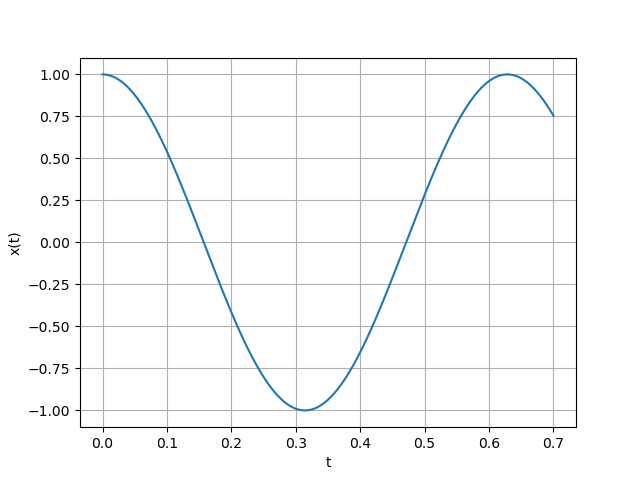
\includegraphics[width = 9cm]{Figure_1}
    Fig. 0. Plot of x\brak{n} \\
    \end{center}
\end{figure}

The ROC of x\brak{n} is defined as the range of values of z for which X\brak{z} will converge where X\brak{z} is the z transform of x\brak{n}.\\
\begin{align}\label{eq:eq10}
   \lvert X\brak{z}\rvert = \sum_{n = -\infty}^{\infty}\lvert x\brak{n}z^{-n}\rvert < \infty
\end{align}

By equation \eqref{eq:eq4} :\\
\begin{align}
X\brak{z} &=  7\sbrak{\sum_{n=0}^{\infty}z^{-n}} + 6\sbrak{\sum_{n=0}^{\infty}nz^{-n}} \label{eq:eq7}
\end{align}
The sum $ \brak{\sum_{n=0}^{\infty}z^{-n}} $ will converge only if z is not zero and $ |z^{-1}|< 1 $ as it is forming an infinite GP with common difference $z^{-1}$. 

Similarly for $\sum_{n=0}^{\infty}nz^{-n}$ to converge, we must have $|z^{-1}| < 1$

Hence, for $X_{1}\brak{z}$ to converge, we must have \\ $|z^{-1}| < 1$ or $|z| > 1$.

\large\textbf{Answer} : \normalsize The ROC of $X_{1}$\brak{z} is  $\lvert z \rvert > 1$

\vspace{4mm}

\large\textbf{\brak{ii}} \normalsize The graph of $x_{2}$\brak{n} is :

\vspace{4mm}

\begin{figure}[!ht]
    \begin{center}
    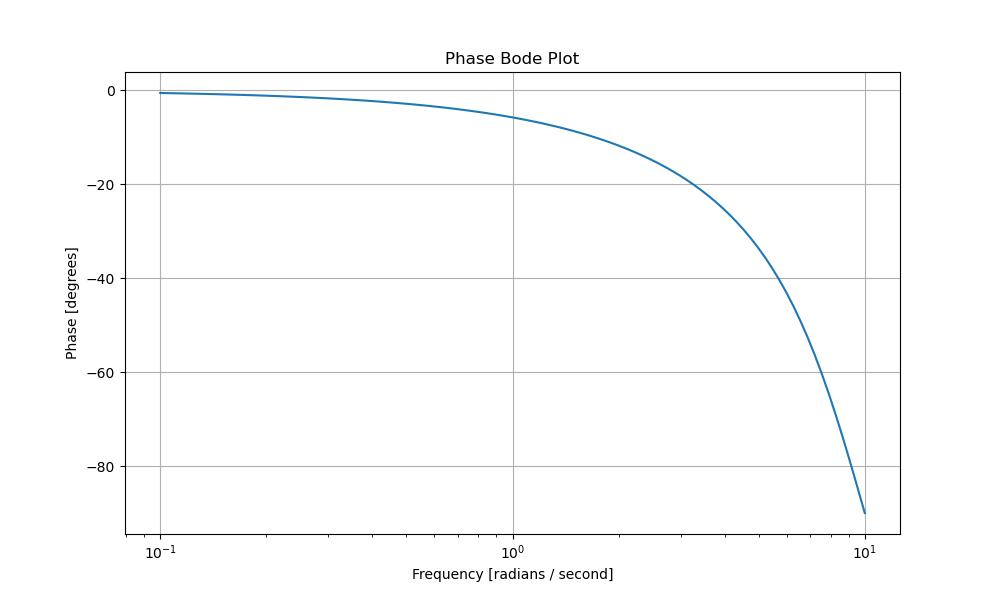
\includegraphics[width = 9cm]{Figure_2}
    Fig. 1. Plot of x\brak{n} \\
    \end{center}
\end{figure}

\FloatBarrier


By equation \eqref{eq:eq8} :\\
\begin{align}
X\brak{z} = 18\sbrak{\sum_{n=0}^{\infty}z^{-n}} - \brak{2\frac{1}{2}}\sbrak{\sum_{n=0}^{\infty}nz^{-n}} \label{eq:eq9}
\end{align}

ROC is given by equation \eqref{eq:eq10}

The sum $ \sbrak{\sum_{n=0}^{\infty}z^{-n}}$ will converge only if z is not zero and $\left|z^{-1}\right| < 1$ as it is forming an infinite GP with common difference $z^{-1}$.\\

Similarly for $\sum_{n=0}^{\infty}nz^{-n}$ to converge, we must have $|z^{-1}| < 1$

Hence, for $X_{2}\brak{z}$ to converge, we must have $|z^{-1} < 1|$ or $|z| > 1$.

\vspace{4mm}

\large\textbf{Answer} : \normalsize The ROC of $X_{2}$\brak{z} is  $|z| > 1$

\end{document}
